%
% TU/e Style Master Thesis template for LaTeX
%
% Public version 1.0
% 2010 - 2013 Thijs Nugteren and Joos Buijs
%
% THIS IS THE MAIN FILE (i.e. compile this file, compiling the others directly won't work)
%
\documentclass[a4paper,10pt,twoside]{report}

%all the other includes etc. are done in the thesis.sty file.
\usepackage{thesis}

%
% These commands need to be defined in order to produce a correct and personalized document
%
\newcommand{\shortdoctitle}{Master's Thesis}
\newcommand{\doctitle}{Efficient Graph Processing Using AWS S3}
\newcommand{\docsubtitle}{Master Thesis}

\newcommand{\me}{Aditya Chandla}
\newcommand{\keywords}{Graph Databases, Serverless}
\newcommand{\version}{1.0}
\newcommand{\monthYear}{July 2024}

%Be sure to use all the titles for your committee members!!! (their names show up on the very first page!)
\newcommand{\firstCommitteeMember}{dr. Nikolay Yakovets}
%\newcommand{\secondCommitteeMember}{Your second Committee Member, usually the daily supervisor}
%\newcommand{\thirdCommitteeMember}{Your Third Committee Member, usually the external member}

\author{\me}

%
% PDF settings
%
\hypersetup
{
    pdfauthor={\me},
    pdftitle={\shortdoctitle},
    pdfsubject={\doctitle},
    pdfkeywords={\keywords}
}

\begin{document}

%use this include for PDF and distribution versions
\pagenumbering{roman}
\begin{titlepage}
\begin{center}

\includegraphics[height=2cm]{figures/tue-logo-high}\\
%\LARGE
%Eindhoven University of Technology \\
\large
Department of Mathematics and Computer Science  \\
Database Group

\vspace*{10cm}

\setlength{\TPHorizModule}{1mm}
\setlength{\TPVertModule}{\TPHorizModule}
% Set the Paragraph Indent to zero, so the first line is not Indented
% Back-up the current value so it can be put back at the end of the title page
\newlength{\backupparindent}
\setlength{\backupparindent}{\parindent}
\setlength{\parindent}{0mm}			
% Begins a textbox at 72 mm from the left of the edge of the paper and 89 mm from the top
% The width of the textbox is 95 mm (167 - 72 mm)
% The height of the box cannot be defined, so it is your task to keep the text not too long
\begin{textblock}{95}(62,89)
    \vspace*{1mm}
    \huge
    \textbf{\doctitle \\}
    \Large
    \vspace*{5mm}
    \textit{\docsubtitle}\\
    \vspace*{10mm}
    \Large
    \me\\
\end{textblock}

\large
Supervisors:\\
\begin{tabular}{rl}
    \firstCommitteeMember\\
    \secondCommitteeMember\\
    \thirdCommitteeMember\\
\end{tabular}

%\vfill
%\version

\vfill
%\docdate \\
\large
Eindhoven, \monthYear\\

% Put the Paragraph Indent back to its original value
\setlength{\parindent}{\backupparindent}
\end{center}
\end{titlepage} 


\normalsize

\clearemptydoublepage

%Sometimes line numbers are nice, uncomment the next line to enable:
%\linenumbers

%It could be handy to have a list of todos and brainstorms in your thesis
%\chapter*{*General todos*}\todo{remove this chapter}
%\input{chapters/general_todos}

%\chapter*{*Brainstorm results*}\todo{remove this chapter}
%\input{chapters/brainstorm_results}

\chapter*{Abstract}\label{chapter:abstract}
As the size of graphs being queried by graph databases increases, coupling 
storage and compute increases the cost and limits the flexibility of
traditional graph database management systems (GDBMS). As part of this thesis,
we explore the viability of an architecture where the compute and storage are
independent. This independence is achieved using a distributed cloud storage
service (AWS S3) which provides bottomless storage and theoretically unlimited
throughput. Using this distributed cloud storage solution, we evaluate the
latency of running two common graph traversal algorithms i.e breadth first
search (BFS) and depth first search (DFS). We then compare this latency with
some other systems which may be used to perform BFS and DFS on large datasets. 
Finally, we provide concrete use cases where using such a decoupled system might
be better suited. 


\clearemptydoublepage

%An executive summary if you want:
%\chapter*{Executive summary}\label{chapter:executive_summary}
%\input{chapters/executive_summary}

%\clearemptydoublepage


\chapter*{Preface}\label{chapter:preface}
Please write all your preface text here. If you do so, don't forget to thank your supervisor, other committee members, your family, colleagues etc.\ etc. 

\clearemptydoublepage

\tableofcontents

\clearemptydoublepage

\listoffigures

\clearemptydoublepage

\listoftables

\clearemptydoublepage

\lstlistoflistings

\clearemptydoublepage

\chapter{Introduction}\label{chapter:introduction}
\setcounter{page}{0}
\pagenumbering{arabic}
%from here on, start the 'real' page numbering, from 1, with normal digits
This is a demo \LaTeX template you can use for your TU/e Master of Science thesis. It can of course also be used for theses at other universities (be sure to use a high quality picture!!!) and other types of theses.

In this particular template special care has been taken to position the thesis title correctly on the front page for the TU/e see-through box in the default cover. However, please check (and double check!) if this is still correct before you send your thesis to the repro shop and have copies printed. Additionally, we defined the command \textbackslash todo\{\} that produces a \todo{The ToDo note} ToDo note in the margin (and introduces some white space in the text unfortunately).

Good luck with your thesis and be sure to share the end result with us on \url{joosbuijs.wordpress.com}!

\vspace{10pt}

Joos Buijs

Eindhoven,

March 2013.

\clearemptydoublepage

\chapter{Preliminaries}\label{chapter:preliminaries}
This template has been used to publish the thesis of Buijs~\cite{MScBuijs2010} and is originally used for the thesis of Nugteren~\cite{MScNugteren2010}. 

One of the best resources for \LaTeX basics, and advanced constructs, is the \LaTeX wikibook\footnote{To be found at~\url{http://en.wikibooks.org/wiki/LaTeX/}}. Of course colleagues and a good internet search using your favorite search engine can do wonders if you're stuck. 

\clearemptydoublepage

\chapter{Experimental Evaluation}\label{chapter:experimentalEvaluation}
Experimental Evaluation
\section{System Architecture}\label{sec:sysArch}
\section{Query Evaluation}\label{sec:queryEvaluation}
\section{Baseline Implementation}\label{sec:baseline}
\section{Improving graph access service}\label{sec:impGraphAccess}
\subsection{Modifying CSR structure}
\subsection{Caching}
\subsection{Prefetching}
\section{Prallelizing graph algorithm service}\label{sec:parallelAlgorithms}
\subsection{Parallel BFS implementation}
\subsection{Parallel DFS implementation}
\section{Optimizing partition sizes}\label{sec:partitionSize}


\clearemptydoublepage

\chapter{Comparisons}\label{chapter:comparisons}
\section{Neo4j}\label{sec:neo4j}
\subsection{Local query evaluation}
\subsection{Distributed query evaluation}
\section{Apache Flink}\label{sec:flink}


\clearemptydoublepage

\chapter{Conclusion and Future Work}\label{chapter:conclusions}
Write your conclusions here.

\clearemptydoublepage

%Choose a good bibliography style, plain would do often, but these might be nice too
%\bibliographystyle{these}
\bibliographystyle{plain}
\bibliography{./references}

\clearemptydoublepage

\appendix
\addcontentsline{toc}{chapter}{Appendix}

\chapter{SNB Schema} \label{sec:schema}
\begin{figure}[ht]
    \centering
    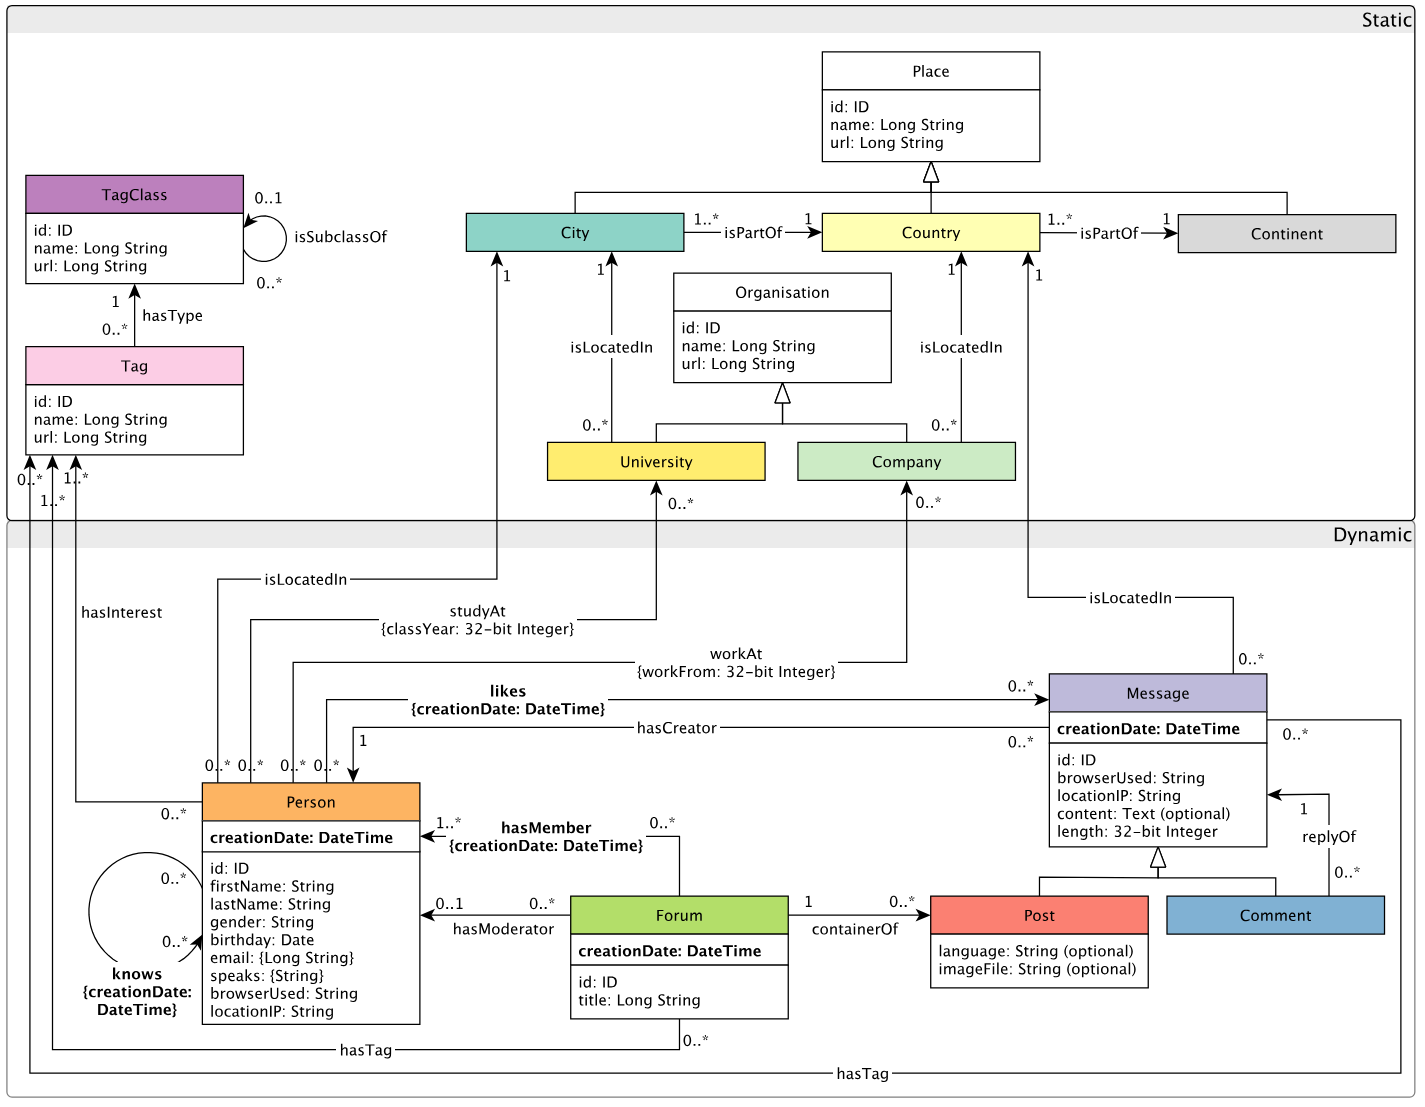
\includegraphics[width=0.9\textwidth]{figures/LDBC-Schema}
    \caption{LDBC SNB Schema}
    \label{fig:ldbcSchema}
\end{figure}
Figure \ref{fig:ldbcSchema} contains the schema of the dataset that was used in
this thesis. This schema along with the underlying dataset was generated as per
the specifications of the LDBC social network benchmark\cite{angles2020ldbc}.


\end{document}
